In this section, we study the implications of 
communication among VMs in colocated and dispersed 
placement scenarios. 
Although the study reveals that there are differences in CPU
utilization based on the placement scenarios, however the exact
CPU utilization levels are incidental to (i) the operating system
versions, (ii) the virtualization technology used and its version,
(iii) the physical machines used and their configurations.
%, and hence
%we do not claim generality in terms of their quantifications.


\subsection{Experimental setup}
\label{sec:arescue-setup}

\begin{figure}[t]
\centering
\subfloat[Xen setup]{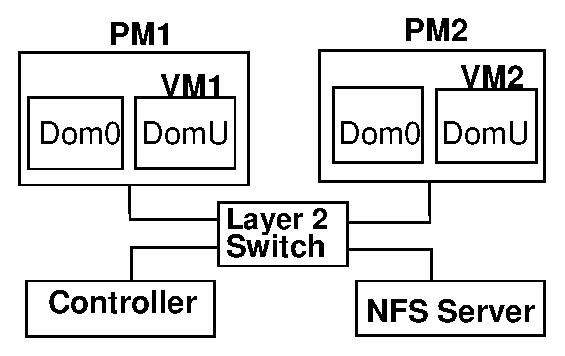
\includegraphics[scale=0.695]{jss-figures/benchmark}} 
~~~~~~~~~~~~~~~~~~~~
\subfloat[KVM setup]{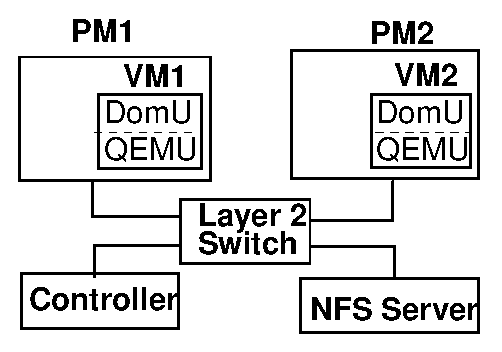
\includegraphics[scale=0.695]{jss-figures/kvmbenchmark}}
\caption{Setup for benchmarking, profiling and model evaluation.}
\label{fig:setup}
\end{figure}
Fig.~\ref{fig:setup} shows the experimental setup that we used. 
The setup used for benchmarking with Xen virtualization technology
is as shown in Fig.\ref{fig:setup}(a) wherein Dom0 is the privileged
domain as described earlier in Section~\ref{sec:litreviewchap-io-virtualization}. 
In case of KVM platform, 
there is no management domain since it
does not follow the driver domain I/O model. Hence, the setup
for KVM benchmarking is a slightly modified version, as
depicted in Fig.~\ref{fig:setup}(b).

As shown in the setup of Fig.~\ref{fig:setup}, two PMs (both with same 
configurations) host the VMs. Each PM
is connected via a Layer-2 Switch to an NFS server which hosts
disk images associated with the VMs. Thus, all disk read/write
operations are NFS-read/write operations which generate network traffic
at the host. The Controller is responsible
for coordination of load generation and resource-usage measurements 
on the VMs.
Load generation is done using an automated script residing at the Controller,
that invokes a custom application program (called \texttt{LoadGen})
at each VM.
For logging of resource utilization, we adopt the ``black-box''
approach~\cite{sandpiper}, i.e, we monitor VM's resource usage by measuring 
only at the hosts (PMs) and not inside the VMs.
% and not within the VMs themselves.
Resource utilization logging is done on the host, using utilities like
\texttt{sar}~\cite{sar}, \texttt{Xentop}~\cite{xentop} (for Xen), 
\texttt{top}~\cite{top} (for KVM) and 
\texttt{iptables}~\cite{iptables}.

The two physical machines hosting the VMs are Intel Core 2
Quad (Q9550) machines with 2.83 GHz cores. Xen version is
3.2 with Linux kernel 2.6.24-26 and KVM version is kvm-62
having QEMU PC emulator version 0.9.1.
%  and are dual-booting
% with Xen 3.2 virtualization environment and KVM module installed in Linux
% kernel version 2.6.24-26.
Both Controller and NFS server (not virtualized, hence common to 
both Xen and KVM setups) are Intel Core 2 (E7400) machines with 
2.60 GHz cores.
The Layer-2 Switch and all network links of the
machines operate at 100 Mbps.


\subsection{Workload generation}
\label{sec:arescue-workloadgen}
As part of our experimental evaluation, we generate 
different types of workloads for benchmarking and
model building.
Workloads are generated using a generic client-server setup,
wherein a \textit{client}
(the controller machine) remotely connects to 
the \textit{servers} (each PM or Dom0,
and VM or DomU). % where workload is to be generated. 
The workload generation
tool resides on each such ``server'' and complies with the 
load generation
requests received from the ``client'' machine. 
Referring to Fig.~\ref{fig:setup}, the 
workload generation requests are sent by the ``Controller''
and VM1/VM2 execute benchmarks to generate the 
requested resource utilization levels. 

Though more detail regarding the design, implementation
and usage of the load generation tool (called \texttt{LoadGen})
is presented in Appendix~\ref{chap:thesis-loadgen}, here 
we mention the different workloads briefly.
The different types of workloads generated by \texttt{LoadGen} are,
% 
% \textbf{SSS:Write up about micro-benchmarks. Also, mention
% the exponential number of cases to consider for combinational loads, and hence
% the randomized choice of combinational load cases.}
\begin{itemize}
\item \textbf{CPU-intensive workloads.}
CPU intensive workloads are generated by having a worker
thread calculate a Fibonacci series with varying periodicity.
If $T$ is the average time for a round of Fibonacci series calculation,
CPU load of $X\%$ is generated by having the worker thread perform
computations for $X \times T$ milliseconds (\emph{active period}) and
sleep for ($100-X) \times T$ milliseconds (\emph{sleep period}).
\item \textbf{Mutable and immutable network-intensive workloads.} 
We generate various levels of network traffic between a pair of VMs by using
a TCP-based custom application that sends a string of bytes on a
TCP socket with different periodicity.
For network workloads, we assume the maximum available capacity 
to be $100$ Mbps and vary the load on each VM by steps 
of $10$ Mbps, from $10$ to $90$ Mbps.
\item \textbf{Disk read \& write workloads.}
We generate disk read (or write) workload by reading (or writing) files  
of $4 kB$ size, with varying intervals to achieve different read access
rates ranging from 0 to 1500 blocks/second. Translating into Mbps, these
rates range from 0 to 5120 Mbps.
\item \textbf{Combination workloads.}
Combination or mixed workloads are generated using 
the same procedures as described above, with a 
multi-threaded process executing different workloads 
simultaneously.
\end{itemize}
As part of the experimental setup, we ensured that for each 
experiment, all combinations of workloads over all VMs do not 
saturate capacity of any resource, i.e., CPU utilization and 
I/O utilization levels are always less than 100\% in all experiments.

\subsection{Effect of colocation on CPU usage}
In this section, we empirically observe the effect of colocation
on CPU resource usages of both Dom0 and DomU. 
By design, we generate the ``same'' load (type and 
amount) for each experiment in both the configurations\textemdash{}dispersed and 
colocated\textemdash{}and observe the differences in actual resource utilization
levels. 
We are interested in addressing the following questions,
(i) For mutable network workloads, is there a decrease in CPU usage when
VMs are colocated, as compared to when they are dispersed? 
(ii) For pure CPU-intensive workloads, is the colocated Dom0 CPU usage
a simple summation of the individual (or dispersed) Dom0 usages, (iii) For
disk read \& write workloads, and immutable network workloads, is
the resultant colocated CPU usage a summation of usages in dispersed
scenarios?

%\begin{figure}%
%\hspace{-0.3in}
%\subfloat[DomU CPU utilization for Rx]{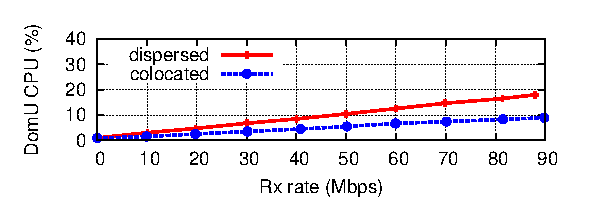
\includegraphics[scale=0.9]{arescue-figures/aff-benchmark/domU-cpu-vs-affine-rx-curve.eps}}
%\subfloat[DomU CPU utilization for Tx]{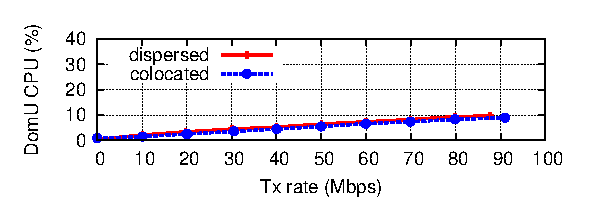
\includegraphics[scale=0.9]{arescue-figures/aff-benchmark/domU-cpu-vs-affine-tx-curve.eps}} \\
%\centering
%\subfloat[Dom0 CPU utilization for Rx/Tx]{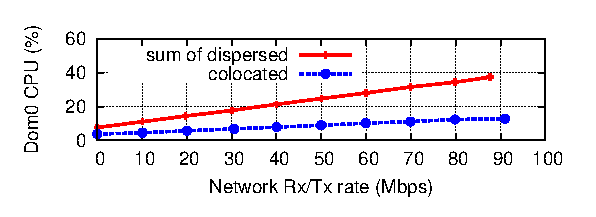
\includegraphics[scale=0.9]{arescue-figures/aff-benchmark/dom0-cpu-vs-affine-curve.eps}}%
%\caption{CPU utilization due to intra-PM network traffic (in Xen setup).}
%\label{fig:cpuovhd-rxtx}
%\end{figure}

%from 2ndchap-benchmark.tex
\begin{figure}[t]%
	% \centering
	\hspace{-0.3in}
	\subfloat[Dispersed DomU CPU utilization for Tx]{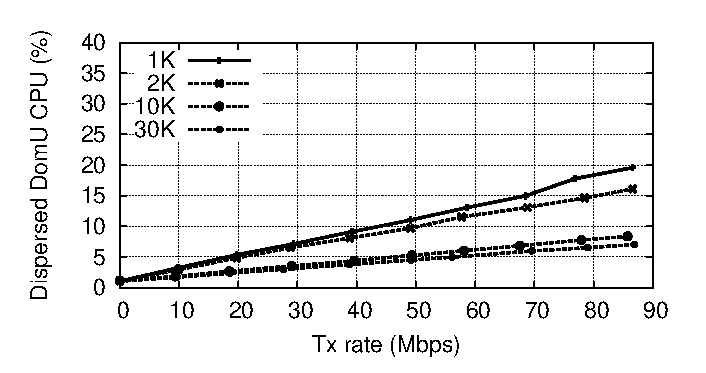
\includegraphics[scale=0.75]{jss-figures/new-aff-benchmark/domu-disp-cpu-for-tx-diff-file-sizes-notsoboth.eps}} ~~
	\subfloat[Colocated DomU CPU utilization for Tx]{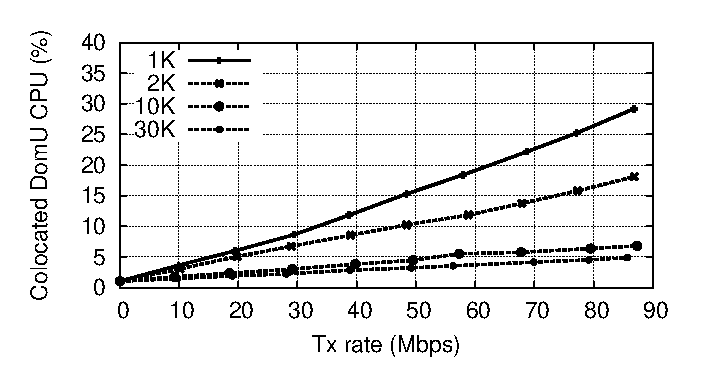
\includegraphics[scale=0.75]{jss-figures/new-aff-benchmark/domu-colo-cpu-for-tx-diff-file-sizes-notsoboth.eps}}
	\caption{CPU utilization due to mutable transmit traffic in dispersed and colocated scenarios with different segment sizes (in Xen setup).}
	\label{fig:xendomutx-chunks}
\end{figure}

\begin{figure}%
	% \centering
	\hspace{-0.3in}
	\subfloat[Dispersed DomU CPU utilization for Rx]{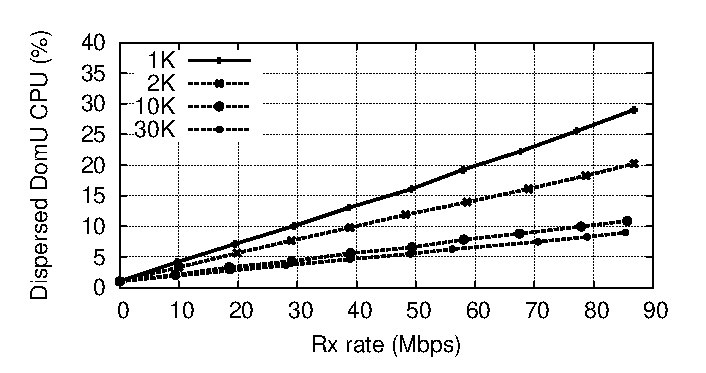
\includegraphics[scale=0.75]{jss-figures/new-aff-benchmark/domu-disp-cpu-for-rx-diff-file-sizes-notsoboth.eps}} ~~
	\subfloat[Colocated DomU CPU utilization for Rx]{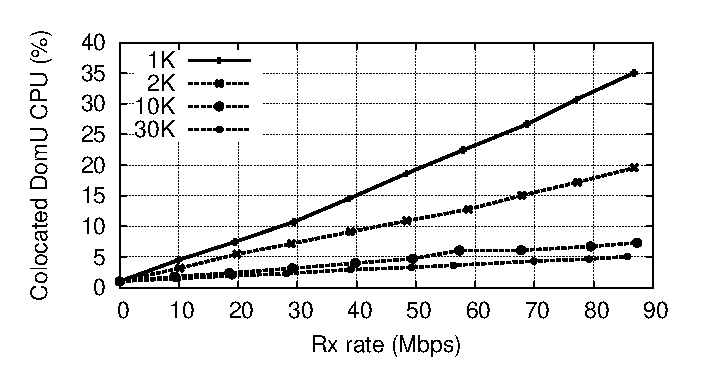
\includegraphics[scale=0.75]{jss-figures/new-aff-benchmark/domu-colo-cpu-for-rx-diff-file-sizes-notsoboth.eps}}
	\caption{CPU utilization due to mutable receive traffic in dispersed and colocated scenarios with different segment sizes (in Xen setup).}
	\label{fig:xendomurx-chunks}
\end{figure}

\begin{figure}[t]
	% \centering
	\hspace{-0.3in}
	\subfloat[Dispersed summation Dom0 CPU utilization for Rx/Tx]{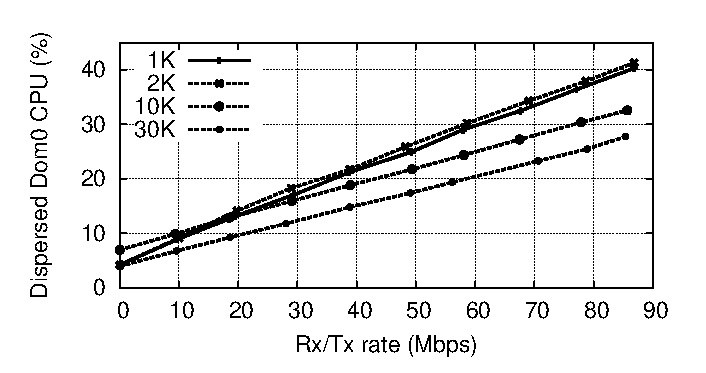
\includegraphics[scale=0.75]{jss-figures/new-aff-benchmark/dom0-dispsum-cpu-for-rxtx-diff-file-sizes-notsoboth.eps}} ~~
	\subfloat[Colocated Dom0 CPU utilization for Rx/Tx]{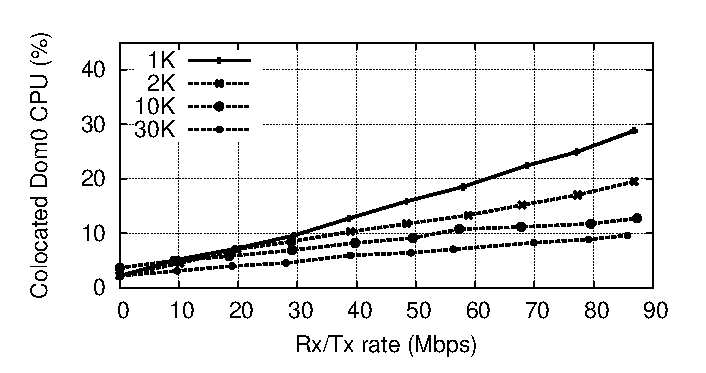
\includegraphics[scale=0.75]{jss-figures/new-aff-benchmark/dom0-colo-cpu-for-rxtx-diff-file-sizes-notsoboth.eps}}
	\caption{CPU utilization for mutable network traffic with different segment sizes (in Xen setup).}
	\label{fig:dom0rxtx}
\end{figure}

\paragraph{I. Impact of mutable network traffic in Xen.} 
One of our claims (and as also discussed 
in~\cite{virtual-putty}, \cite{starling}),
is that colocated provisioning can result in changes in
resource usage for mutually communicating VMs. % and availability. 
% `Affine' traffic refers to the network communication
% within the VM pair under consideration.
In this experiment, VM1
and VM2 act as a Tx/Rx pair to transmit and receive data
at different rates, such that
VM1 is the transmitting DomU\index{DomU}
and VM2 is the receiving DomU.
To study the implications of mutable network-affinity
between VMs, the experiment is conducted in both 
colocated and dispersed scenarios, and CPU utilization for
DomU (and Dom0 in Xen) is measured.
In our setup, we observed that TSO (TCP Segmentation
Offload)\nomenclature{TSO:}{TCP Segmentation Offload}\index{TSO} feature was
enabled whereas the complementary feature LRO (Large
Receive Offload)\nomenclature{LRO:}{Large Receive Offload}\index{LRO} at
receiving end
was not functional. For the sake of
uniformity at both transmitting and receiving ends, we disabled
TSO for our experiments.

Fig.~\ref{fig:xendomutx-chunks}(a) and \ref{fig:xendomutx-chunks}(b)
plot the transmitting DomU's CPU utilization for varying usage
of network bandwidth in Xen\index{Xen} setup. Each line represents
the use of a different application-level segment size
(sizes are mentioned in the legend).
As described in Section~\ref{sec:arescue-background}, inter-PM and
intra-PM communication have different execution paths,
hence resulting in different CPU utilization.
As can be seen, for higher segment sizes, increase
in network bandwidth usage results in higher CPU savings upon
colocation. However, the opposite result is
observed for smaller segment sizes.
The bold lines in the graph represent those
segment sizes for which colocated CPU usage is higher than
dispersed whereas the dotted lines indicate those having
colocated CPU usage as lower than dispersed. For example,
for the segment size of 30KB at 80Mbps network utilization,
CPU utilization is 8\% for dispersed and 4.8\% for colocated,
thus indicating a drop of approximately 3\% absolute CPU
when transitioning into colocated. On the other other hand,
for the segment size of 1KB at 85Mbps, CPU utilization
is 29\% for dispersed and 35\% for the colocated scenario,
which indicates a 6\% increase while moving into colocated placement.
A similar result was observed for the receiving DomU as well,
as depicted in Fig.~\ref{fig:xendomurx-chunks}.

Fig.~\ref{fig:dom0rxtx} shows Dom0 CPU utilization
levels for two communicating VMs,
with
\ref{fig:dom0rxtx}(a)
showing the summation of the two dispersed Dom0 CPU utilization
and
\ref{fig:dom0rxtx}(b)
showing the colocated Dom0 utilization.
We can see that in all cases,
the summation utilization is significantly greater than the
colocated Dom0 utilization. For example,
for the segment size of 30KB at 80Mbps network utilization,
the difference in absolute Dom0 CPU usage between
dispersed (summation of utilization at both Dom0's in the
dispersed scenario) and colocated (single
Dom0 CPU) scenarios is 16\% and similarly for 2KB segment size,
this difference is around 20\% absolute CPU.
The above observations suggest that not only the bit-rate of
transmission, but also the segment size affects CPU utilization
in both colocated and dispersed scenarios, and we need to consider
both these factors while modeling CPU usage. Further, we also
observe that in all above experiments, CPU usage varies linearly
with respect to network utilization.


% This implies that there is definitely
% no increase in CPU utilization due to colocation of two 
% communicating VMs.
%Further, the absolute usage by Rx-network traffic is more
%than Tx-traffic for the same bandwidth\textemdash{}CPU utilization
%of 17\% and 9\% respectively, at 90 Mbps network bandwidth
%utilization.
%Fig.~\ref{fig:cpuovhd-rxtx}(c) shows the Dom0 CPU utilization
%levels for two communicating VMs.
%Comparing network rates of 40 Mbps and 90 Mbps,
%the difference in absolute Dom0 CPU usage between
%dispersed (summation of utilization levels at both PMs in the
%dispersed scenario) and colocated (single
%Dom0 CPU) scenarios is 14\% and 25\%, respectively.

%when both the Rx/Tx network traffic is between colocated VMs.
%Considering network utilization of 85 Mbps, Dom0's CPU
%requirements is about 12\%.
%{\bf Dom0 plot should have dom0-non-co-hosted-rx as well. 
%the colocated scenario is plotting dom0-cpu-rxtx ... ?}

\begin{figure*}[t]%
	\centering
	\subfloat[Dispersed Guest VM CPU utilization for Rx]{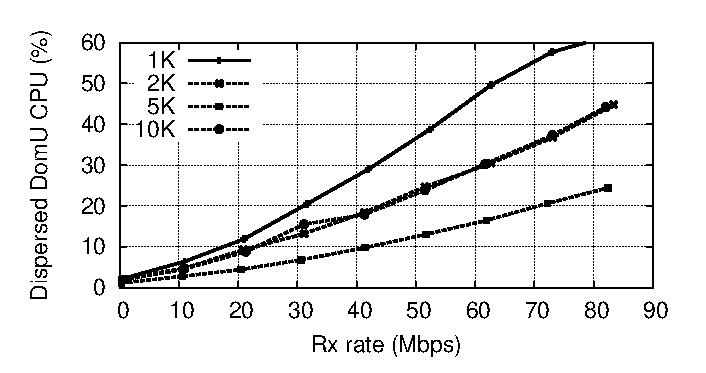
\includegraphics[scale=0.75]{jss-figures/kvm-aff-benchmark/domu-disp-cpu-for-rx-diff-file-sizes-notsoboth-kvm.eps}} ~~
	\subfloat[Colocated Guest VM CPU utilization for Rx]{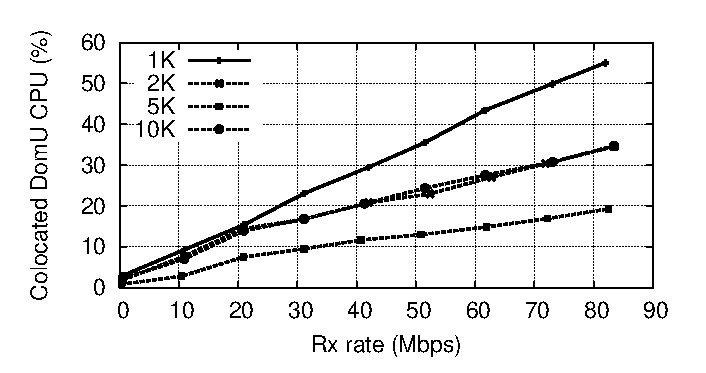
\includegraphics[scale=0.75]{jss-figures/kvm-aff-benchmark/domu-colo-cpu-for-rx-diff-file-sizes-notsoboth-kvm.eps}}
	\caption{CPU utilization for mutable receive traffic with different segment sizes (in KVM setup).}
	\label{fig:kvmdomurx-chunks}
\end{figure*}

\begin{figure*}[t]%
	\centering
	\subfloat[Dispersed Guest VM CPU utilization for Tx]{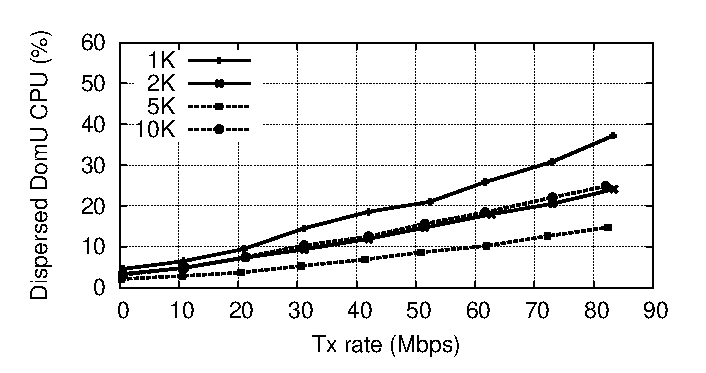
\includegraphics[scale=0.75]{jss-figures/kvm-aff-benchmark/domu-disp-cpu-for-tx-diff-file-sizes-notsoboth-kvm.eps}} ~~
	\subfloat[Colocated Guest VM CPU utilization for Tx]{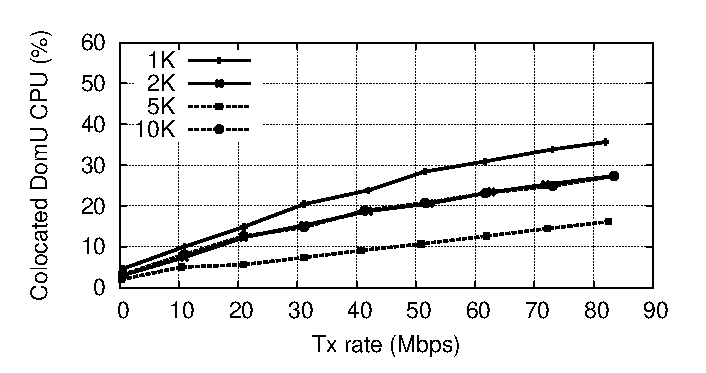
\includegraphics[scale=0.75]{jss-figures/kvm-aff-benchmark/domu-colo-cpu-for-tx-diff-file-sizes-notsoboth-kvm.eps}}
	\caption{CPU utilization for mutable transmit traffic with different segment sizes (in KVM setup).}
	\label{fig:kvmdomutx-chunks}
\end{figure*}

\paragraph{II. Impact of mutable network traffic in KVM.}
\label{sec:2ndchap-kvm-benchmark}
Similar to the benchmarking for Xen presented above, we performed
an empirical study of colocation effects in KVM as well.
As mentioned earlier, KVM does not have the concept of a privileged
domain to arbitrate I/O access amongst the VMs. Instead, each VM
is similar to a process and invokes the QEMU\index{QEMU} emulator to
access the
I/O devices. Thus, the overhead related to I/O processing (and the
resulting effects due to dispersed and colocated network
communication) would be reflected in the VM (DomU) CPU usage itself.
Fig.~\ref{fig:kvmdomurx-chunks} and Fig.~\ref{fig:kvmdomutx-chunks}
show CPU utilization
of the DomUs in dispersed and colocated scenarios in KVM\index{KVM}
setup. The experiment setting is such that VM1 requests varying
network rates in the range 10 to 80Mbps for
% (when VM1 requests, it plays
% the receiving domain role and VM2 is the transmitting domain) 
each segment size while VM2 requests a fixed rate of 10Mbps.
Thus, though both VMs are transmitting and
receiving data, the variations in network rate at a given
segment size setting are caused only by VM1's request-rate.

Fig.~\ref{fig:kvmdomurx-chunks} shows that when receive traffic
at VM1 is 80Mbps for a segment size of 10KB, DomU CPU usage is
44\% absolute CPU in dispersed case and drops to 35\% in colocated case
whereas for segment size of 1KB, CPU usage drops from 62\% in
dispersed case to 55\% in colocated case. Similarly,
Fig.~\ref{fig:kvmdomutx-chunks}
shows CPU usage plots for VM2 transmitting 80Mbps using
%the transmitting domain for 
various
segment sizes. Thus, we observe that CPU usage of transmitting
and receiving DomUs change between colocated \& dispersed scenarios.
Additionally, we also observe that CPU utilization
is approximately linear with respect to network utilization in
above experiments.


%%%%%%%%%%%%%%%%%%%%%%%%% nonaff-rx
\begin{table}
\caption{Percentage CPU usage for \textit{immutable} Rx.}
\centering
% \noindent\makebox[\textwidth]{% 
\begin{tabular}{|c|c|c|} \hline
\textbf{Immutable} & \multicolumn{2}{|c|}{\textbf{Percentage CPU utilization}} \\ \cline{2-3} \cline{2-3}
\textbf{Receive} & \textbf{Dispersed case} & \textbf{Colocated case} \\
(Mbps) & $VM_1,VM_2, \sum Dom0_i$ & $VM_1,VM_2,Dom0$ \\ \hline
% $<$20, 10$>$ & 3, 2, 12 & 3, 2, ~8 \\ \hline
% $<$20, 30$>$ & 4, 5, 14 & 3, 5, 11 \\ \hline
$<$20, 50$>$ & 4, 7, 18 & 4, 7, 14 \\ \hline
$<$20, 70$>$ & 4, 9, 21 & 4, 9, 17 \\ \hline
$<$40, 10$>$ & 6, 2, 15 & 6, 2, 11 \\ \hline
$<$40, 30$>$ & 7, 5, 18 & 7, 5, 15 \\ \hline
$<$40, 50$>$ & 7, 7, 21 & 7, 7, 18 \\ \hline
$<$60, 10$>$ & 8, 2, 18 & 8, 2, 14 \\ \hline
% $<$60, 30$>$ & 8, 5, 21 & 8, 5, 18 \\ \hline
\end{tabular}
% }
%\caption{Non-affine receive benchmarking results for colocated provisioning}
\label{nonaff-rx-benchmark}
%\vspace{-0.3in}
\end{table}

\paragraph{III. Other workloads.}
Table~\ref{nonaff-rx-benchmark} shows colocated benchmarking
results for immutable \textit{receive} traffic\textemdash{}VMs receiving 
network packets from ``dispersed'' (i.e. hosted on different PMs) transmitters. 
The table shows CPU usage of VMs in
dispersed and colocated cases for Dom0 and DomU.
The left most column shows tuples of the form $<x,y>$ where
$x$ is the the receive rate at VM1 and $y$ is the receive
rate at VM2. The second column shows the CPU utilization of 
VM1, VM2 and the summation of the CPU utilization of the two 
Dom0 instances in dispersed scenario. The third column shows
the CPU utilization of VM1, VM2 and the single Dom0 instance
in the colocated scenario.
Observe that
DomU CPU utilization stay similar in both dispersed \& colocated
cases.
The colocated Dom0
CPU utilization is consistently (4\%) less than 
the summation of the Dom0 utilization
levels in the dispersed case.

Similar observation was made for other workloads\textemdash{}immutable
transmit traffic, CPU workloads, disk read and disk write workloads. 
The Dom0 utilization of 4\% is the same as its utilization
under idle load, hence the above observation implies that for all
other workloads except mutable traffic, colocation results in saving
the CPU overhead related to an extra Dom0 instance.
%More detailed results can be found in the related technical report 
%at \cite{affine-modeling-tech-report}.

\paragraph{IV. Summary of benchmarking}
From the benchmarking phase, we have following take-aways,
\begin{itemize}
  \item When the nature of mutable network traffic changes between intra-PM
				  and inter-PM, there
				  is a change in guest VM CPU utilization in both Xen
				  and KVM environments. 
				  %, and this change is dependent on not only the
%				  network rate but also the application segment size.
  \item In case of Xen Dom0, change in nature of network-affinity results
				  in significant change (up to 25\% absolute CPU) when comparing
				  colocated Dom0 against the summation of dispersed Dom0 utilization.
  \item With increase in network utilization, 
	  the increase in CPU utilization is linear
			 in both Xen and KVM environments.
	\item For all workloads, other than mutable network traffic, colocation results
		in similar DomU CPU usages in both colocated and dispersed cases.
	\item For all workloads, other than mutable network traffic, the summation of CPU 
		usage of the two Dom0 instances in dispersed case differs from the 
		colocated CPU usage by a constant amount (say 4\% absolute CPU). 
\end{itemize}
		  
\textit{Based on the results of benchmarking, we
			  conclude that the relation between increase in network utilization
		  and CPU utilization is linear for both Xen and KVM environments.}
		  \footnote{These results are applicable only when both the network
			  and CPU resources have spare capacity, e.g., if CPU utilization is
			  already close to 100\%, increasing the network rate is either not
			  possible or results in no corresponding change in CPU utilization.
			  All further observations, modeling and inferences are based on this
		  premise.} As a result, both the ``total'' as well as 
		  the ``differences'' in CPU utilization can be
		  captured using linear estimation models.


%\paragraph{III. Summary of Xen benchmarking with colocation.}
%From the above set of benchmarking experiments, 
%we conclude that 
%For mutable network traffic, there is
%marginal reduction in DomU CPU utilization after colocation and
%significant savings (up to 25\%) in Dom0 CPU utilization.

%clipped 10feb
\subsection{Feasibility of Generic models}
In order to build a model that can be generically used to
predict CPU utilization of DomUs, 
even though it is trained on only one or couple of VMs,
it is necessary that VMs behave similarly under
similar loading conditions. 
For example, suppose a CPU load of
$x\%$ is requested, but creates $x+5\%$ CPU load on one VM.
%As mentioned before, this accuracy is enough for our benchmark
%profiling, however, 
It is essential that the same load when
requested on another homogeneous VM, results in similar
resource utilization levels. 
% This is a very basic expectation
% % and we present some sample results to demonstrate that this
% % does indeed hold. 
Thus, we are interested in verifying the 
following two hypotheses\textemdash{}(i) Given similar 
configurations, CPU utilization for similar load levels on 
different VMs match up, (ii) Given similar platforms, CPU 
utilization for similar loads on same VM but different PMs match up.
 
To this end, we performed several repeatable experiments 
on two VMs that were placed in a dispersed manner and compared whether 
similar loads result in similar CPU utilization levels on both VMs
and their Dom0s. We performed such experiments for all load 
types\textemdash{}CPU intensive, mutable traffic, immutable traffic
and disk-intensive\textemdash{}and as expected, we observed that both the
above hypotheses about CPU utilization on different VMs 
and PMs held true.
\\
\\
In this section, we established the basic benchmarking results that
will be applied to develop a generic CPU estimation model. By generic,
we imply that a single model would be able to estimate CPU utilization
for any given application, without requiring re-training on the specific
application itself.
In the next section, we present our approach to develop the generic
model and use it to estimate the CPU usage when a pair
of VMs are colocated or dispersed.

